
%=====================================================================
%CAPITULO I
%=======================================================================
\chapter{Conjuntos}
\marginnote{
\begin{center}
 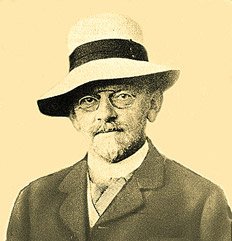
\includegraphics[scale=.4]{imagenes/Hilbert.jpg}\\
\end{center}
\small
<<David Hilbert (Königsberg, Prusia Oriental; 23 de enero de 1862-Gotinga, Alemania; 14 de febrero de 1943) fue un matemático alemán, reconocido como uno de los más influyentes del siglo XIX y principios del XX. Estableció su reputación como gran matemático y científico inventando y/o desarrollando un gran abanico de ideas, como la teoría de invariantes, la axiomatización de la geometría y la noción de espacio de Hilbert, uno de los fundamentos del análisis funcional. Hilbert y sus estudiantes proporcionaron partes significativas de la infraestructura matemática necesaria para la mecánica cuántica y la relatividad general. Fue uno de los fundadores de la teoría de la demostración, la lógica matemática y la distinción entre matemática y metamatemática. Adoptó y defendió vivamente la teoría de conjuntos y los números transfinitos de Cantor. Un ejemplo famoso de su liderazgo mundial en la matemática es su presentación en 1900 de un conjunto de problemas abiertos que incidió en el curso de gran parte de la investigación matemática del siglo XX.>> (Wikipedia)
}
\begin{quote}
 <<Nadie nos expulsará del paraíso que \index[personas]{Cantor} Cantor ha creado para nosotros>> 
\end{quote}
\begin{flushright}
 David Hilbert \index[personas]{Hilbert}
\end{flushright}






En esta unidad estudiaremos el concepto de
\index{Conjuntos!cardinal}\emph{cardinal} de un conjunto. Con este concepto se pretende dar
un significado a la noción de cantidad de elementos de un
conjunto, en especial cuando este es ``infinito''. Como se verá,
y por extraño que parezca, aunque el conjunto involucrado sea
infinito de todas maneras podremos definir el cardinal de ese
conjunto. Con esto implicitamente decimos que no todos los
conjuntos infinitos tendrán el mismo cardinal. Empezaremos
recordando algunas cuestiones básicas de teoría de
conjuntos que, a la vez, nos servirán como referencia para  las
notaciones.

%--------------------------------------------------------------
%SECCION




\section{Repaso nociones básicas sobre \index{Conjuntos} conjuntos}
La siguiente introducción está lejos de ser exhaustiva, solo
recordaremos conceptos ya sabidos. Nos dentendremos algo más en
aquellos puntos que puedan ser nuevos.

\begin{definicion}Dados dos conjuntos $A$ y $B$ denotaremos su \index{Conjuntos!union}\index{Conjuntos!intersección}\index{Conjuntos!diferencia}\emph{unión,
intersección y diferencia} por: $A\cup B$, $A\cap B$ y $A-B$
repectivamente. Estos nuevos conjuntos se definen por: \index[simbolos]{$A\cup B$}\index[simbolos]{$A\cap B$}\index[simbolos]{$A-B$}
\[A\cup B=\{x:x\in A\vee x\in B\},\]

\[A\cap B=\{x:x\in A\wedge x\in B\}\]
y

\[A-B=\{x:x\in A \wedge x\notin B\},\]
respectivamente.
\end{definicion}
 Por lo general, tendremos que los
conjuntos con los que trabajaremos estarán contenidos en un
conjunto que llamaremos el universo $\mathcal{U}$. Aceptado la
existencia de este universo, frecuentemente usaremos la siguiente
notación para el \emph{complemento} 
\[A^c=\mathcal{U}-A.\] 
\index[simbolos]{$A^c$}
Además consideraremos la operación de \index{Conjuntos!diferencia simétrica}\emph{diferencia simétrica},
definiéndose por:
\[A\bigtriangleup B=(A-B)\cup(B-A).\]
\index[simbolos]{$A\bigtriangleup B$}
\begin{definicion}Dados dos elementos arbitrarios $a$ y $b$ se
define el \emph{par ordenado}\index{par ordenado} $(a,b)$, por la siguiente igualdad
\[(a,b)=\{a,\{a,b\}\}.\]
\end{definicion}

La propiedad más relevante de pares ordenados es que si \index[simbolos]{$(a,b)$}
$(a,b)=(c,d)$ entonces $a=c$ y $b=d$. Eso se infiere de la demostración y queda como ejercicio. Ahora consideramos el
conjunto formado por todos los pares ordenados de elementos
pertenecientes a conjuntos dados.

\begin{definicion} Sean $A$ y $B$ conjuntos. El \index{Conjuntos!producto cartesiano}\emph{producto cartesiano} de $A$ con
$B$, denotado por $A\times B$, es el siguiente conjunto:
\[A\times B=\{(a,b):a\in A\wedge b\in B\}.\]
\end{definicion}
La siguiente definición es bien conocida.

\begin{definicion} Una \index{Función} \emph{función} $f$ de $A$ en $B$ (abreviaremos esta frase
porel siguiente símbolo: $f:A\longrightarrow B$)\index[simbolos]{$f:A\longrightarrow B$}, es un
subconjunto del producto cartesiano $A\times B$ con la propiedad
que: para todo $a\in A$ existe un único $b\in B$ tal que
$(a,b)\in f$. \end{definicion}

Suponemos que ya todos conocemos estos conceptos, asi como los
conceptos relacionados de: imagen, la notación $f(a)$, función
inyectiva, suryectiva y biyectiva. Admitimos todo esto por sabido.
Ahora introducimos una nueva notación.

\begin{definicion}
Por $B^A$ \index[simbolos]{$B^A$} denotamos al conjunto de todas las funciones
$f:A\longrightarrow B$.
\end{definicion}

Mas adelante daremos algunas explicaciones del porque de esta
notación.

Seguidamente damos las definiciones de los conjuntos imagen y preimagen de un conjunto dado por una función.

\marginnote{
\begin{center}
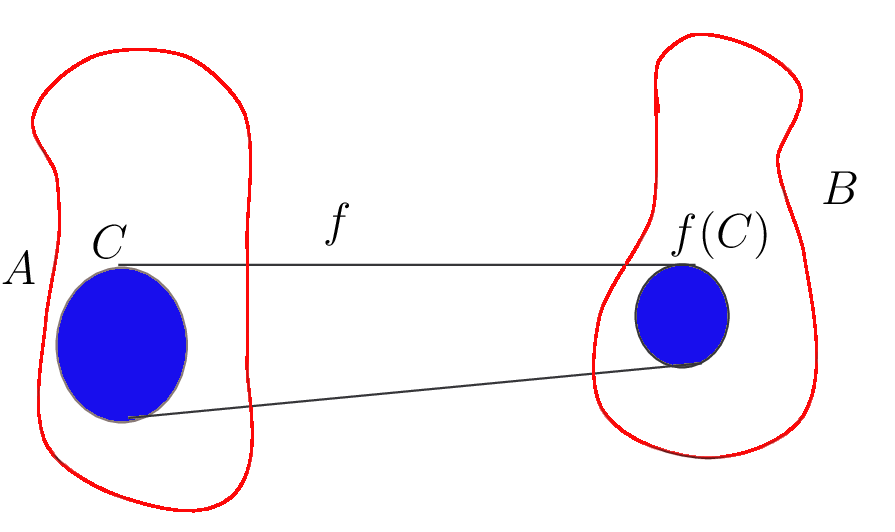
\includegraphics[scale=.15]{imagenes/funcima.png}\\
Conjunto $f(C)$
\end{center}
}
\begin{definicion} Dada una función $f:A\longrightarrow B$ y subconjuntos
$C\subset A$ y $D\subset B$ definimos:
\[f(C)=\{f(a):a\in C\}\]
y
\[f^{-1}(D)=\{a\in A:f(a)\in C\}.\]
\end{definicion}
\marginnote{
\begin{center}
 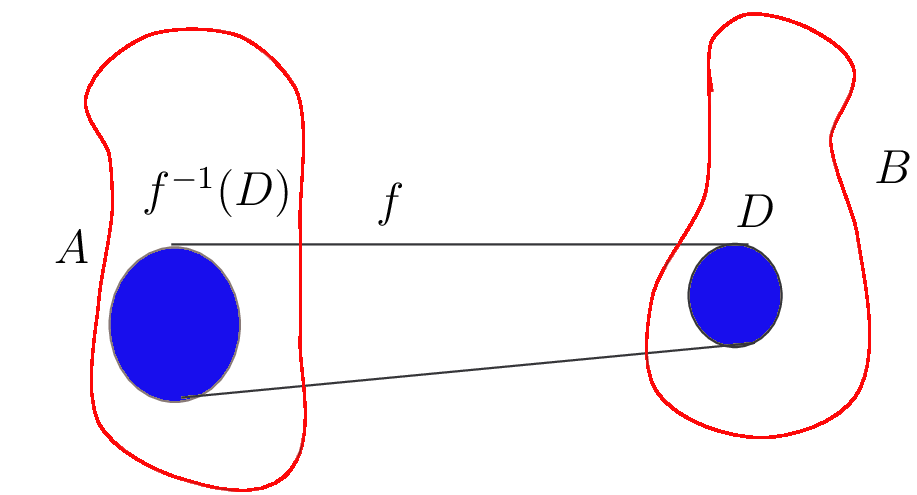
\includegraphics[scale=.15]{imagenes/fpreima.png}\\
 Conjunto $f^{-1}(D)$
\end{center}
}











Muy a menudo utilizaremos las propiedades que a continuación se
enuncian. Las demostraciones, de las mismas, quedaran a cargo del
alumno; ver Ejercicio \vref{3}.

\begin{proposicion}\label{propfunc} Sea $f:A\longrightarrow B$ una función.
Entonces
\begin{itemize}
\item[1.] $f(C_1\cup C_2)=f(C_1)\cup f(C_2).$
\item[2.]$f^{-1}(D_1\cup D_2)= f^{-1}(D_1)\cup f^{-1}(D_2).$
\item[3.] $f(C_1\cap C_2)\subset f(C_1)\cap f(C_2).$
\item[4.]$f^{-1}(D_1\cap D_2)= f^{-1}(D_1)\cap f^{-1}(D_2).$
\end{itemize}
\end{proposicion}


También vamos a considerar el \index{Conjuntos!partes}\emph{conjunto de partes} de un conjunto
dado, esto es el conjunto de todos sus subconjuntos.
Explícitamente:
\[\mathcal{P}(A)=\{C:C\subset A\}.\]
Se pueden efectuar uniones e intersecciones de una cantidad
arbitraria de conjuntos. Para poder enunciarlas debemos definir
antes lo que entendemos por una \emph{familia subindicada de
conjuntos} (o brevemente \emph{familia de conjuntos}).

\begin{definicion} Supongamos dado un conjunto $I$, al que nos referiremos como
conjunto de índices, y una función $i:I\longrightarrow
\mathcal{P}(A)$. Así tenemos que, para cada $i\in I$, existe
un único subconjunto de $A$, que llamaremos $A_i$. Diremos entonces que $\{A_i\}_{i\in I}$ es una familia
subindicada de conjuntos por el conjunto de índices $I$.
\end{definicion}

Ahora podemos definir la unión y la intersección de una
familia de esta índole de la siguiente manera
\begin{definicion} Definimos la unión e intersección de una
familia $\{A_i\}_{i\in I}$ por:
\[\bigcup_{i\in I}A_i=\{a:\exists i\in I:a\in A_i\}\]\index[simbolos]{$\bigcup_{i\in I}A_i$}
y
\[\bigcap_{i\in I}A_i=\{a:\forall i\in I:a\in A_i\}\]\index[simbolos]{$\bigcap_{i\in I}A_i$}
respectivamente.
\end{definicion}
En el Ejercicio \vref{propuniarb} podemos encontrar una serie de
propiedades de uniones e intersecciones de familias de conjuntos.
Estas propiedades las usaremos con frecuencia.
 Por último, en esta revisión de conjuntos, expondremos el
 axioma de elección. Este es un axioma de la teoría de
 conjuntos. Hay que aclarar que es posible axiomatizar la
 teoría de conjuntos, de esta axiomatización el mencionado axioma
 puede formar parte. Decimos ``puede'' por que este
 axioma ha despertado multitud de controversias en torno a su
 inserción o no en el restante conjunto de axiomas. No vamos a
 discutir aquí esta controversia ni tampoco la teoría
 axiomática de conjuntos pues esto nos desviaría de nuetros
 objetivos. Solo enunciaremos el \index{Axioma de elección}\emph{axioma de elección}, que
 usaremos frecuentemente.

\begin{axioma} Sea $\{A_i\}_{i\in I}$ una familia de conjuntos no
vacios. Entonces existe una función
\[f:I\longrightarrow\bigcup_{i\in I}A_i.\]
con la propiedad  que: 
\[\forall i\in I: f(i)\in A_i.\]
\end{axioma}



%--------------------------------------------------------------
%SECCION


\section{Definición de conjuntos coordinables}\marginnote{\vspace{-6cm}
\begin{center}
 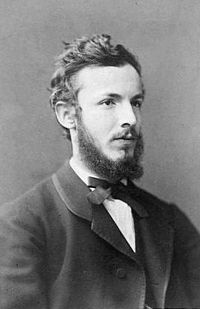
\includegraphics[scale=.4]{imagenes/Cantor.jpg}\\
 George Cantor (1845-1918)
\end{center}
\small
Georg Ferdinand Ludwig Philipp Cantor (San Petersburgo, 3 de marzo de 1845-Halle, 6 de enero de 1918) fue un matemático y lógico nacido en Rusia. Fue inventor con \index[personas]{Dedekind}\index[personas]{Frege}Dedekind y Frege de la teoría de conjuntos, que es la base de las matemáticas modernas. Gracias a sus atrevidas investigaciones sobre los conjuntos infinitos fue el primero capaz de formalizar la noción de infinito bajo la forma de los números transfinitos (cardinales y ordinales). 
(Wikipedia)}
En esta sección definimos el concepto clave de esta unidad, a
saber el concepto de que dos conjuntos sean \index{Conjuntos!coordinabilidad}\emph{coordinables}. Este concepto fue introducido y explotado por George Cantor.  Damos
una breve discución para motivar nuestra definición.

 Cuando
alguién cuenta algún conjunto de cosas, establece una
correspondencia entre los objetos que cuenta y un subconjunto de
números naturales. En el proceso de conteo,
algún objeto fue el primero en contarse, y se habrá dicho:
``uno'' para ese objeto. El proceso continua asignando,
sucesivamente, el número dos, tres, etc, a los restantes objetos
a contar, hasta que no queden más por contarse. Así, si en
este proceso llegamos hasta el 20, por ejemplo, decimos que hay 20
objetos. Aunque no haya que percatarse de eso a los fines
prácticos, lo que también hicimos fue establecer una
correspondencia o función entre los objetos y el conjunto
$\{1,\dots,20\}$. Más aún, esta correspondencia fue biyectiva
pues a cada número le correspondió solo uno de los objetos, es decir la función es inyectiva, y a cada objeto le
correspondió algún número, es decir  la función es
suryectiva. En otras palabras contar un conjunto significa
determinar el \index{intervalo inicial} \emph{intervalo inicial} del conjunto de los
números naturales para el cual exista una correspondencia biyectiva
con el conjunto que queremos contar. Conocer esto obviamente es
inútil a los efectos de contar cosas de la ``vida cotidiana'';
no obstante, es una observación fundamental a los efectos de
extender lo que llamamos ``contar'' a conjuntos infinitos. Lo que
antecede sugiere la siguiente definición.
\marginnote{ \emph{Intervalo inicial:}  un conjunto de
la forma: $\{j\in\mathbb{N}:1\leq j\leq n\}$, para cierto
$n\in\mathbb{N}$. De ahora en más, llamaremos a este conjunto:
$\mathbb{N}_n$}
\begin{definicion}\label{defcoordinables} Dados dos conjuntos: $A$ y $B$,
se dirá que ellos son coordinables, escribiremos \index[simbolos]{$A\thicksim B$}$A\thicksim B$,
si existe una función biyectiva $f:A\longrightarrow B$.
\end{definicion}

Esta es nuestra definición de que dos conjuntos, finitos o
no, tengan la misma cantidad de elementos. Como veremos, no
todos los  conjuntos infinitos son coordinables entre si. 
Es bueno notar que no es difícil demostrar que $\thicksim$ es
una relación de equivalencia (ver Ejercicio \vref{1}).
 Ahora
veamos algunos ejemplos.

\begin{ejemplo}Consideremos la función
$f:\nn\longrightarrow\{x\in\nn:x\,\,\text{es par}\}$, definida por
$f(x)=2x$. Facilmente se ve que $f$ es una biyección entre los
conjuntos indicados. De ahí que:
$\nn\thicksim\{x\in\nn:x\,\,\text{es par}\}$.
\end{ejemplo}

En este ejemplo observamos que, desde nuestro punto de vista, el
conjunto de los naturales tiene la misma cantidad de elementos
que el conjunto de los naturales pares. Es decir, según nuestra concepción de cantidad de elementos, el
todo no es mayor que una de sus partes. Este ejemplo ya lo había mencionado Galileo Galilei.

\begin{ejemplo}\label{rcoord(0,1)} Veamos que $\rr\thicksim (0,1)$. En este caso se
puede considerar la función

\[f(x):= \tan\biggl(\frac{2\pi x-\pi}{2}\biggr).\]
Dejamos como ejercicio corroborar que la función dada establece
una biyección entre los conjuntos involucrados.
\end{ejemplo}

Los dos ejemplos anteriores muestran una característica
importante de los conjuntos infinitos; un subconjunto de ellos
puede ser coordinable con el conjunto total. Mientras que, los
conjuntos finitos  carecen de esta característica.
Ver Ejercicio \vref{infcoordconsub}




%--------------------------------------------------------------
%SECCION

\section{Conjuntos numerables}
Hasta el momento hemos hablado de conjuntos
finitos e infinitos. Apelamos a la idea que todos nos forjamos en nuestras vidas  sobre el significado de estos términos .  Pero en este momento estamos  en condiciones, a
partir de la noción  de coordinalidad, de definir de forma
matemáticamente precisa los anteriores  significados.
\index{Conjuntos!finitos}\index{Conjuntos!infinitos}\index{Conjuntos!numerables}\index{Conjuntos!a lo sumo numerables}
\begin{definicion} Diremos que un conjunto $A$ es:
\begin{itemize}
\item[1.] \textbf{finito} si existe un $n\in\nn$ tal que
$A\thicksim\nn_n$.
\item[2.] \textbf{infinito }si no es finito.
\item[3.] \textbf{numerable} si $A\thicksim\nn$.
\item[4.] \textbf{a lo sumo numerable} si es finito o numerable.
\end{itemize}
\end{definicion}

En virtud de que $\thicksim$ es una realción de equivalencia, y
especialmente por el carácter transitivo de esta, si $A\thicksim
B$ y $B$ tiene alguna de las cuatro propiedades de la definición
anterior entonces $A$ tendrá esa misma propiedad.

Recordemos que, por definición, una sucesión $\{a_i\}$ de
elementos de un conjunto $A$ es una función
$f:\nn\longrightarrow A$, donde $a_i=f(i)$. Vemos así que el
concepto de numerabilidad está relacionado con el de sucesión.
En efecto, si el conjunto $A$ es numerable entonces sus elementos
se pueden disponer en una sucesión, donde ningún término se
repita.

Es oportuno que observemos que un conjunto no puede ser numerable
y finito a la vez; dicho de otra forma, los conjuntos numerables
son infinitos. Esto, como hemos definido los conceptos numerable y
finito de  manera precisa, tiene que ser demostrado.

\begin{teorema}\label{nesinfinito} Un conjunto numerable es
infinito.
\end{teorema}
\begin{demo} Supongamos que, por lo contrario, existe un conjunto
$A$ numerable y, a la vez, finito. Así tendríamos que:
$A\thicksim\nn$ y $A\thicksim\nn_n$, para algún $n\in\nn$. Como
$\thicksim$ es una relación de equivalencia , deducimos que
$\nn\thicksim\nn_n$. Sea, pues, $f$ una biyección:
$f:\nn_n\longrightarrow\nn$. Ahora consideremos el
natural\footnote{El símbolo $:=$ se lee \emph{igual por
definición}. Esto es, el miembro de la izquierda es definido por
el de la derecha}: $k:=f(1)+\dots+f(n)+1$. Como $f$ es una
biyección, existe algún $m$, con $1\leq m\leq n$ tal que
$f(m)=k$. Es decir
\[f(m)=f(1)+\dots+f(n)+1.\]
Seguramente, en el miembro derecho, uno de los términos es
$f(m)$. Este se puede cancelar con el miembro de la izquierda,
quedando
\[0=f(1)+\dots+f(m-1)+f(m+1)+\dots+f(n)+1.\]
Esta igualdad es absurda pues el miembro de la derecha es mayor
que $1$.
\end{demo}

Vamos a ver algunos otros conjuntos que también son numerables.
Empezamos por el siguiente.

\begin{proposicion}\label{subconjunto} Un subconjunto de un conjunto a lo sumo numerable es a
lo sumo numerable.
\end{proposicion}
\begin{demo} Sea $A\subset B$, con $B$ a lo sumo numerable. Se puede suponer
que $B\subset \nn$. ?`Por qué? Y, también podemos suponer que
$A$ es infinito, puesto que si fuera finito no habría nada
que probar. Definimos una función $f:\nn\longrightarrow A$ por
induccion. Puesto que los números naturales son bien ordenados,
tenemos que $A$ tiene un primer elemento, digamos, $a_1$.
Definamos
\[f(1)=a_1.\]
Ahora definimos $f(j)$ por:
\begin{equation}\label{frecursiva}
f(j)=\text{el primer elemento del conjunto: }A-\{f(i):1\leq i\leq
j-1\}. \end{equation} Esta definición es posible pues
$A-\{f(i):1\leq i\leq j-1\}\neq\emptyset$, de lo contrario $A$
sería finito. Queda así definida la función $f$. Resta
ver que es biyectiva.

Veamos, en primer lugar, que es inyectiva. Sea $i>j$. En virtud de
~\eqref{frecursiva}, tenemos que $f(i)\notin\{f(k):1\leq k\leq
i-1\}$ de lo cual, y como $j<i$, deducimos que $f(i)\neq f(j)$.

Ahora veamos la suryectividad. Supongamos que existe un elemento
$n\in A$ tal que $n\notin f(\nn)$. Recordemos la Definición
\eqref{frecursiva}. Ella nos dice, en virtud de que $n\notin
f(\nn)$, que $f(i)<n$, para todo $i$. Esto es debido a que $f(i)$
es el mínimo del conjunto $ A-\{f(k):1\leq k\leq i-1\}$ y a
que $n$ pertenece a ese conjunto. Tenemos, entonces, que
$f(\nn)\subset\nn_n$. Como consecuencia del Ejercicio \vref{1.5}
concluímos que $f(\nn)$ es finito. Pero como $f$ es inyectiva
$\nn\thicksim f(\nn)$. Lo que es una contradicción pues $\nn$ es
infinito.
\end{demo}

\begin{proposicion}\label{zesnum}
El conjuntos $\mathbb{Z}$, de los enteros,  es numerable.
\end{proposicion}
\begin{demo} Construímos una función que establece
una biyección entre los enteros positivos y los naturales pares
y entre los enteros negativos y los naturales impares. La
función es la siguiente:

\[f(x)=\left\{
\begin{array}{ll}
    2x+2, & \hbox{si $x\geq 0$;} \\
    -2x-1, & \hbox{si $x<0$.} \\
\end{array}
\right.\] Dejamos como ejercicio demostrar que, efectivamente, la
función $f$ es una biyección entre $\nn$ y $\mathbb{Z}$.
\end{demo}

\begin{proposicion}\label{NxNesnum} El conjunto $\nn\times\nn$ es numerable.
\end{proposicion}
\begin{demo} La demostración de este enunciado ya no es tan
sencilla. La idea se la debemos a G. Cantor. Primero presentaremos un razonamiento \href{https://es.wikipedia.org/wiki/Heur%C3%ADstica}{heurístico}  de
la construcción de la biyección entre $\nn\times\nn$
 y $\nn$. En rigor de verdad, a los efectos lógicos de la demostración, toda esta parte de la demostración
 se podría obviar; pudiéndose dar la fórmula
 ~\eqref{forfinal} sin dar ninguna justificación de como se nos
 ocurrió. Elegimos el camino contrario, explicar
 como obtener la fórmula.


 Dispongamos del conjunto $\nn\times\nn$ en un arreglo del tipo
de una ``matríz infinita'', como sigue:
\[\begin{diagram}
(1,1)   & \rTo        & (1,2)  &                      & (1,3)  &                      & (1,4) &\dots\\
        & \ldTo(2,2)  &        &\ldTo(2,2)\ruTo(4,2)  &        & \ldTo(2,2)\ruTo(6,4) &        &     \\
(2,1)   &             & (2,2)  &                      & (2,3)  &                      &        &      \\
        &\ldTo(2,2)   &        & \ldTo(2,2)           &        & \ddots               &        &      \\
(3,1)   &             &(3,2)   &                      &        &                      &        &      \\
        & \ldTo(2,2)  &        &   \ddots             &        &                      &        &      \\
 (4,1)  &             &        &                      &        &                      &        &      \\
 \vdots &             &        &                      &        &                      &        &      \\
\end{diagram}\]
Notar que, además de colocar los pares ordenados, hemos colocado
algunas flechas. Estas flechas indican un camino. Este es el
camino que seguiremos  para enumerar los pares ordenados.
Así, construiremos una función $f$ que hará las
siguientes asignaciones:

\begin{eqnarray}
    f:\nn\times\nn&\longrightarrow\nn\nonumber \\
    (1,1)&\longmapsto 1\nonumber \\
    (1,2)&\longmapsto 2\nonumber \\
     (2,1)&\longmapsto 3\nonumber\\
        &\hspace{-29pt}\vdots\nonumber \\
        \nonumber
\end{eqnarray}
Observar que en nuestro camino vamos siguiendo diagonales de
la matriz, de izquierda a derecha y de arriba hacia abajo. Cuando llegamos al margen izquierdo de la matriz
saltamos al borde superior, para luego descender por la
siguiente diagonal. Estas diagonales tienen $1, 2, 3, \dots$
elementos. Agrupemos los números naturales de esa forma, es
decir un primer grupo de uno, un segundo de dos y así
sucesivamente:

\[\underbrace{1}_{1} \underbrace{2\quad 3}_{2}\quad\underbrace{4\quad 5\quad
6}_{3}\quad \underbrace{7\quad 8\quad  9\quad 10}_{4}\dots
\]
Obsérvese que

\begin{equation}\label{numfinal}
\frac{j(j +1)}{2}=\text{número final del agrupamiento
$j$-ésimo}.
\end{equation}
Por ejemplo: el grupo cuarto tiene por su último elemento el 10,
que es igual a 4.5/2. Tambien tenemos que todos los pares
ordenados sobre la misma diagonal, tienen la característica
de que sus componentes suman lo mismo. Numeremos las diagonales,
de izquierda a derecha, empezando por 1. Así tenemos que la
diagonal 1 posee el elemento (1,1), la diagonal dos tiene los
elementos $(1,2)$ y $(2,1)$, etc. Por lo observado, tenemos la
siguiente fórmula, para cualquier par $(j,k)$

\begin{equation}\label{numdiag}
j+k-1=\text{el número de la diagonal a la que pertenece } (j,k).
\end{equation}
 El objetivo es poner en correspondencia la diagonal
$j$-ésima con el grupo $j$-ésimo de naturales. Notar que, en
virtud de ~\eqref{numfinal}, tenemos que
\begin{equation}\label{numdiag2}
\begin{split}\frac{(j+k-1)(j+k)}{2}=&\text{es el último número}\\
 & \text{del agrupamiento $j+k-1$-ésimo}.\\
\end{split}
\end{equation}
Así, si al primer miembro de ~\eqref{numdiag2} le restamos
$(j-1)$, obtenemos el número que ocupa el lugar $j$ (contando de
atras para adelante) del agrupamiento $j+k-1$ de naturales. Con
esto probamos que la función que queriamos construir es:


\begin{equation}\label{forfinal}
f(j,k):=\frac{(j+k-1)(j+k)}{2}-j+1.
\end{equation}
El resto de la demostración lo dejamos como ejercicio. Es decir la   demostración que ~\eqref{forfinal} es
biyectiva (ver Ejercicio \vref{2}).
\end{demo}

Como consecuencia del Ejercicio \vref{1.2} y de la Proposición
anterior, podemos afirmar que si $A$ y $B$ son numerables,
entonces $A\times B$ es numerable.



La siguiente propiedad también es útil para determinar si un
conjunto es numerable.

\begin{proposicion}\label{numinysur}Sean $A$ y $B$ conjuntos, con $B$ a lo sumo
numerable.
\begin{itemize}
\item[1.] Supongamos que existe una función inyectiva $f:A\longrightarrow
B$. Entonces $A$ es a lo sumo numerable.
\item[2.] Supongamos que existe una aplicación suryectiva
$f:B\longrightarrow A$. Entonces $A$ es a lo sumo numerable.
\end{itemize}
\end{proposicion}
\begin{demo} Veamos primero 1. La función $f$ es  una biyección entre $A$ y su
imagen $f(A)$. Como $B$ es a lo sumo numerable,  y como
consecuencia de la Proposición \vref{subconjunto}, tenemos que
$f(A)$ es a lo sumo numerable. Ahora, como $A\thicksim f(A)$
tenemos que $A$ es a lo sumo numerable.

Ahora probemos 2. Como $f$ es suryectiva, tenemos que $\forall
a\in A$: $f^{-1}(\{a\})\neq\emptyset$. Ahora, por el axioma de
elección sabemos que existe al menos una función
$g:A\longrightarrow B$ tal que $\forall a\in A:g(a)\in
f^{-1}(\{a\})$. Si pudiéramos probar que la función $g$ fuera
inyectiva, entonces obtendríamos la tesis a partir del inciso
1, que ya fue demostrado. Veamos, pues, que $g$ es inyectiva.
Supongamos que $a_1,a_2\in A$ y que $a_1\neq a_2$. Afirmamos que
$f^{-1}(\{a_1\})\cap f^{-1}(\{a_2\})=\emptyset$. En efecto, si
$b\in f^{-1}(\{a_1\})\cap f^{-1}(\{a_2\})$ entonces por un lado
 $f(b)=a_1$ y por otro $f(b)=a_2$, lo que es una contradicción pues $a_1\neq a_2$.
\end{demo}

Es interesante hacer notar que, utilizando el teorema anterior,
podemos dar otra demostración, más concisa, de la
Proposición \vref{NxNesnum}.

En esta demostración hacemos uso del Teorema Fundamental de la
Aritmética. Recordemos lo que este teorema nos dice:


\begin{teorema}[Fundamental de la Aritmética] Todo entero positivo $n$ se representa, de
manera única, de la forma $n=p_1^{\alpha_1}p_2^{\alpha_2}\dots
p_j^{\alpha_j}$, donde $p_1$, $p_2$,...,$p_j$ son números primos
y $\alpha_1$, $\alpha_2$,...,$\alpha_j$ son enteros positivos.
\end{teorema}

\begin{demo} \emph{alternativa de la Proposición \ref{NxNesnum}}
Definimos la siguiente función

\[\begin{split}
f:\nn\times\nn&\longrightarrow\nn\\
 (n,m)&\longrightarrow 2^n3^m\\
 \end{split}.
 \]
Por el Teorema Fundamental de la Aritmética, y mas precisamente
por la unicidad de la representación, tenemos, como $2$ y $3$
son primos, que si $2^n3^m=2^{n^{\prime}}3^{m^{\prime}}$ entonces
$n=n^{\prime}$ y $m=m^{\prime}$. Por consiguiente la función $f$
es inyectiva. Ahora, invocando la Proposición \vref{numinysur}
concluímos que $\nn\times\nn$ es a lo sumo numerable. Lo que
resta es, solo, ver que $\nn\times\nn$ no es finito. Esto se puede
probar observando que $\nn\times\nn$ contiene el subconjunto
$A=\{(1,n):n\in\nn\}$ que es coordinable con $\nn$, ?`Cuál es la
biyección?, y por consiguiente infinito. Así,
$\nn\times\nn$ no puede ser finito, si lo fuera, $A$ también lo
sería, por ser un subconjunto de él. Lo que concluye la
demostración.
\end{demo}

Ahora podemos demostrar  uno de los resultados más interesantes
de esta teoría.

\begin{teorema} El conjunto $\mathbb{Q}$ es numerable.
\end{teorema}
\begin{demo} Sabemos que $\mathbb{Z}$ es numerable y dejamos como ejercicio demostrar que $\mathbb{Z}-\{0\}$ es numerable. Consecuentemente también  $\mathbb{Z}\times\mathbb{Z}-\{0\}$ es numerable. Podemos
definir la siguiente función:
\[
\begin{split}
f:\mathbb{Z}\times\mathbb{Z}-\{0\}&\longrightarrow\mathbb{Q}\\
(n,m)&\longmapsto \frac{n}{m}
\end{split}
.\] Esta aplicación es suryectiva. Por consiguiente, usando la
parte 2. de la Proposición \vref{numinysur}, obtenemos que
$\mathbb{Q}$ es a lo sumo numerable. Así $\mathbb{Q}$ es
finito o numerable. Pero como $\mathbb{Q}$ es infinito, pues
$\nn\subset\mathbb{Q}$, tenemos que $\mathbb{Q}$ es numerable. \end{demo}


Traduciendo nuestra interpretación de que dos conjuntos
coordinables tienen la misma cantidad de elementos, vemos que hay
tantos racionales como naturales. Esta afirmación es un tanto
desconcertante. Sabemos que los racionales son
densos dentro de los reales. Esto quiere decir que dentro de cada
intervalo abierto, por chico que este fuere, siempre hay números
racionales dentro. Sin embargo, uno puede poner en correspondencia
$\nn$ y $\mathbb{Q}$.  

A esta altura pareciera que
todos los conjuntos resultan ser numerables, pero ya veremos, en
la sección siguiente, que no es así.


\begin{lema}\label{subconjnum} Todo conjunto infinito tiene un
subconjunto numerable.
\end{lema}

\begin{demo} Sea $A$ un conjunto infinito. Usaremos un argumento similar a la demostración de
la Proposición \vref{subconjunto}. Definimos inductivamente una
función $f:\nn\longrightarrow A$  de la siguiente manera. Puesto
que $A$ es infinito, en particular, es no vacio, así podemos
encontrar un elemento $a_1\in A$. Ponemos entonces
\[f(1)=a_1.\]
Ahora, supongamos que tenemos definida la función $f$, de tal
manera que sea inyectiva, para $j=1,\dots n$. Llamemos $f(j)=a_j$,
para $j=1,\dots , n$. Como $A$ es infinito no puede ocurrir que
$A-\{f(1),\dots,f(n)\}=\emptyset$, de lo contrario $f$ además de
ser inyectiva, de $\nn_n$ en $A$, sería suryectiva; y de este
modo $A\thicksim\nn_n$ lo que implica que $A$ es finito,
contrariando nuestra hipótesis. Por consiguiente, podemos
encontrar $a_{n+1}\in A-\{f(1),\dots,f(n)\}$. Definimos
$f(n+1)=a_{n+1}$.

Ahora veamos que $f$ así definida es inyectiva. Sea $i\neq
j $, podemos suponer que $i<j$. Sabemos que:
\[f(j)\notin \{f(1),\dots,f(j-1)\}.\]
Seguramente $f(i)$ es un elemento del conjunto de la derecha, en
la relación anterior, de modo que $f(j)\neq f(i)$, lo que
demuestra la inyectividad. Ahora, $f$ es biyectiva de $\nn$ en
$f(\nn)$. Por consiguiente $f(\nn)$ es un subconjunto de $A$
numerable. 
\end{demo}

La siguiente proposición es útil para probar que algunos
conjuntos son numerables. Antes de enunciarla, haremos una
observación útil a la demostración. Afirmamos que si $A$ es
un conjunto a lo sumo numerable, entonces existe una función
suryectiva de $\nn$ en $A$. En efecto, si $A$ es numerable, esto
es claro puesto que existe una biyección de $\nn$ en $A$. Si,
por el contrario, $A$ es finito, entonces existe una biyección
de $\nn_n$, para algún $n\in\nn$, en $A$; en este caso
extendemos la biyección a todo $\nn$ de cualquier
forma\footnote{Por ejemplo: ponemos $f(j)=1$ para $j>n$}, la
función resultante es suryectiva, aunque ya no inyectiva.

\begin{proposicion}\label{unionnumdenum} Sea $I$ un conjunto de índices a lo sumo
numerable. Supongamos que para cada $i\in I$ tenemos un conjunto
$A_i$ que, también, es a lo sumo numerable. Entonces
\[\bigcup_{i\in I}A_i\]
es a lo sumo numerable. Brevemente: ``Una unión a lo sumo
numerable de conjuntos a lo sumo numerables es a lo sumo
numerable''.
\end{proposicion}

\begin{demo} Como vimos, para cada $i\in I$ existe una función
suryectiva $f_i:\nn\longrightarrow A_i$. Definimos:
\[\begin{split}
      f:\nn\times I &\longrightarrow \bigcup_{i\in I}A_i\\
         (n,i)&\longmapsto f_i(n).\\
 \end{split}
\]
Esta función es suryectiva, pues si
\[a\in\bigcup_{i\in I}A_i,\]
entonces $a\in A_{i_0}$, para algún $i_0$; ahora, utilizando la
suryectividad de $f_{i_0}$, obtenemos un $n\in\nn$ tal que
$f_{i_0}(n)=a$. Es decir $f(n,i_0)=a$. Esto prueba que $f$  es
suryectiva. Ahora, como $\nn\times I$ es a lo sumo numerable, en
rigor es numerable, y por la Proposición \vref{numinysur},
obtenemos la tesis.
\end{demo}


\section{Un conjunto no numerable} \index{Conjuntos;no numerables}
Vimos que $\nn$ es numerable, por definición, y que $\mathbb{Z}$
y $\mathbb{Q}$ son también numerables. Ahora mostraremos un
conjunto que no es a lo sumo numerable. No será otro que el
conjunto de los numeros reales.


\begin{teorema}\label{realnonum} El conjunto $\mathbb{R}$ no es
a lo sumo numerable.
\end{teorema}
\begin{demo} Supongamos, por el contrario, que $\mathbb{R}$ es a
lo sumo numerable. En virtud de la Proposición
\vref{subconjunto}, tendríamos que el intervalo $[0,1)$
sería también a lo sumo numerable. Como él es infinito
entonces $[0,1)$ sería numerable. Sea, entonces, una
función biyectiva $f:\nn\longrightarrow [0,1)$. Definamos
$a_j:=f(j)$.

Como es sabido, cada número real $r$ admite un desarrollo en
expresión decimal infinita del tipo

\[r=0.r_1r_2r_3\dots.\]
Un peque\~no inconveniente lo presenta el hecho de que esta
expresión decimal no es única, puesto que, por ejemplo:
$2.000\dots=1.999\dots$. Para avolir este problema convenimos que
en nuestros desarrollos decimales no usaremos expresiones que
tienen todos $9$ a partir de cierto momento. Con esta
convención, el desarrollo decimal es único.

A los fines de clarificar nuestra demostración, es útil poner
a la sucesión $a_j$ de la siguiente manera :
\[\begin{split}
a_1&=0.a_{1,1}a_{1,2}a_{1,3}\dots\\
a_2&=0.a_{2,1}a_{2,2}a_{2,3}\dots\\
\vdots&\\
a_n&=0.a_{n,1}a_{n,2}a_{n,3}\dots\\
 \vdots&\\
 \end{split}\]
Ahora definimos un número $r=0.r_1r_2\dots\in[0,1)$, tomando en
cuenta los valores de $a_{i,j}$ sobre la digonal principal, que
por fuerza no será ninguno de los $a_j$. La definición es la
siguiente:
\[r_n:=\left\{
\begin{array}{ll}
    2, & \hbox{si $a_{n,n}<2$;} \\
    1, & \hbox{si $a_{n,n}\geq 2$.} \\
\end{array}
\right.
\]
Tenemos que $r\neq a_j$ para todo $j$, pues, estos números
seguramente son distintos en el lugar $j$ de su desarrollo.
Observar que si $a_j$ tiene un número menor que 2 en ese lugar,
entonces $r_j=2$, en cambio si un número mayor o igual que 2
ocupa el lugar $j$ de $a_j$, entonces $r_j=1$. Por ende, como
dijimos $r$ no es ningún $a_j$. Esto demuestra que la función
$f$ no es suryectiva.
\end{demo}

Utilizando el Ejemplo \vref{rcoord(0,1)} y el Ejercicio \vref{5},
vemos que $\rr\thicksim (0,1)\thicksim [0,1]$. Para cualquier
intérvalo no trivial\footnote{Por un intérvalo trivial
entendemos un intérvalo que se reduce a un punto} $I$,  ya sea
abierto o cerrado, existe una biyección, de hecho una función
lineal, de $I$ en el intérvalo $(0,1)$ o $[0,1]$, dependiendo de
si $I$ es cerrado o abierto. Vemos así que todos los
intérvalos no triviales son coordinables entre si y a su vez
con $\rr$.



\section{Una aplicación}
En esta sección daremos una aplicación de los conceptos
desarrollados en las secciones previas. Veremos como estos se
pueden usar para demostrar la existencia de números
trascendentes. Antes empezaremos con algunas definiciones.

Un polinomio es una expresión de la forma:
\[P(X)=a_0+a_1X+a_2X^2+\dots+a_nX^n,\]
donde $n\in\nn$ se llama \emph{grado} del polinomio y los $a_j$
\emph{coeficientes} del polinomio.  Escribiremos que $P\in
\mathbb{Z}[X]$, $P\in\mathbb{Q}[X]$ o $P\in\mathbb{C}[X]$ si los
coeficientes son enteros, racionales o complejos respectivamente.
Una raíz del polinomio $P$ es un número
$\alpha\in\mathbb{C}$ tal que
\[P(\alpha)=0.\]

Observar que un número racional $q=n/m$ es solución (o
raíz del polinomio) de la siguiente ecuación:
\[P(X):=mX-n=0.\]
Notar que este polinomio $P$ es de primer grado y además
$P\in\mathbb{Z}[X]$. Reciprocamente, si $q$ es solución de una
ecuación polinomial $P(X)=0$, donde $P$ es de primer grado y con
coeficientes en $\mathbb{Z}$, entonces $q$ es racional.

Hemos aprendido que hay dos clases de reales,\index{Números!racionales}\index{Números!irracionales} \emph{racionales e
irracionales}. En esta sección expondremos otros tipos de
números reales, a saber los \emph{trascendentes}\index{Números!trascendentes}. 


Tomemos por caso el
número $\sqrt{2}$, que como sabemos es irracional. A pesar de
ello $\sqrt{2}$ es solución de una ecuación a coeficientes
enteros de  segundo grado. Nos referimos a
siguiente:
\[X^2-2=0.\]
Vemos que $\sqrt{2}$ tiene, si se nos permite por el momento esta
expresión, un grado de irracionalidad no muy grande, puesto
que es solución de una ecuación de segundo grado a
coeficientes enteros. A estos números se los llama \index{Números!irracionales cuadráticos} \emph{irracionales cuadráticos}.

Nos preguntamos ahora si existiran números que acorde con la perspectiva anterior tengan el mayor grado
de irracionalidad  posible. Esto es que no sean solución de
ninguna ecuación polinomial a coeficientes enteros, no importa
del grado que fuere. Llamaremos a estos números, cuya existencia
es hipotética por el momento, \emph{trascendentes}. A los
restantes números los llamaremos \index{Números!algebraicos} \emph{algebraicos}. Denotaremos
por $\mathbb{A}$ al conjunto de números algebraicos y por
$\mathbb{T}$ al conjunto de números trascendentes. Cualquier
número que sea obtenido por medio de raices, del grado que
fuere, de números enteros son algebraicos. Esto indica que
resolver el problema planteado puede no ser fácil.

El problema de la existencia de números trascendentes fue
resuelto por \index[personas]{Liouville}Liouville en 1844. El demostró que el número
\[L=\sum_{n=0}^{\infty}\frac{1}{10^{n!}}\]
es trascendente. Posteriormente C. Hermite\index[personas]{Hermite} demostró en 1873
que $e=2.7172...$ es trascendente y Lindemann\index[personas]{Lindemann}, en 1882, que $\pi$
también lo es.

En esta sección mostraremos el argumento usado por G. Cantor, en
1874, para demostrar la existencia de números trascendentes. La
situación es la siguiente: Cantor demostró que el conjunto de
los números algebraicos es numerable. Luego, si el conjunto de
los trascendentes lo fuera, también lo sería el conjunto
$\rr$ (unión de dos numerables es numerable), lo cual no es
cierto. Asi es que no solo los números trascendentes existen,
sino que existen tantos como números reales hay. Dicho de otro
modo, los números trascendentes son los más comunes entre los
números reales. Los racionales, por el contrario, son una
excepción, habiendo de ellos solo una cantidad numerable.

Es bueno comentar que hubo matemáticos  que se opusieron a
G.Cantor y a su Teoría de Conjuntos. Quizas la gota que
rebalso el vaso fue la anterior demostración de la existencia
de números trascendentes. Pues es una manifestación de que la 
teoría de Cantor podía ser utilizada para demostrar cuestiones 
matemáticas profundas que no aparentaban tener nada que ver con
la teoría de conjuntos.

La clave de la demostración es el siguiente lema.

\begin{lema} El conjunto $\mathbb{Z}[X]$ es numerable.
\end{lema}
\begin{demo} Un polinomio  en $\mathbb{Z}[X]$ y de grado $n$ se puede
identificar con la $n+1$-upla de enteros formada por sus
coeficientes. Teniendo en cuenta esto, definimos la siguiente
función:
\[\begin{split}
          f:\mathbb{Z}[X]&\longrightarrow
            \bigcup_{n=1}^{\infty}\mathbb{Z}^n\\
            a_0+a_1X+\dots+a_nX^n&\longmapsto (a_0,a_1,\dots,
            a_n)\\
            \end{split},
\]
donde
\[\mathbb{Z}^n:=\underbrace{\mathbb{Z}\times\dots\times\mathbb{Z}}_{n\,\,\text{veces}}.\]
Por lo dicho con anterioridad, esta función es biyectiva.

Ahora bien, el conjunto $\mathbb{Z}^n$ es numerable. Podemos
probar esto usando inducción y el hecho de que el producto
cartesiano de conjuntos numerables es numerable. Así, como
consecuencia de la Proposición \vref{unionnumdenum} obtenemos
que
\[\bigcup_{n=1}^{\infty}\mathbb{Z}^n\]
es numerable. Como $f$ es una biyección, $\mathbb{Z}[X]$ es
numerable.
\end{demo}

Como corolario obtenemos que el conjunto de números algebraicos
es numerable.

\begin{corolario}\label{algsonnum}
El conjunto de números algebraicos es numerable.
\end{corolario}
\begin{demo} Se tiene que
\[\mathbb{A}=\bigcup_{P\in\mathbb{Z}[X]}\{\alpha:P(\alpha)=0\}.\]
Como es sabido de los cursos de álgebra, dado un polinomio $P$,
de grado $n$, el conjunto $\{\alpha:P(\alpha)=0\}$ es finito, es
mas, tiene a lo sumo $n$ elementos. Ahora, en virtud de esto y la
Proposición \vref{unionnumdenum}, obtenemos que $\mathbb{A}$ es
a lo sumo numerable. Ciertamente, este conjunto es infinito, pues
$\nn$ está contenido en él, de modo que no tiene mas chance
que la de ser numerable.
\end{demo}

Como otro corolario  obtenemos que
$\mathbb{T}\neq\emptyset$. Pues de lo contrario, como
$\rr=\mathbb{A}\cup\mathbb{T}$ y como la unión de a lo sumo
numerables es a lo sumo numerable, tendríamos que $\rr$
sería a lo sumo numerable, que es una contradicción. Pero
en realidad podemos demostrar algo más que
$\mathbb{T}\neq\emptyset$; podemos probar que
$\mathbb{T}\thicksim\rr$. Esto es consecuencia del siguiente
teorema, que afirma que al sacarle un conjunto numerable a un
conjunto coordinable con $\rr$ no alteramos la cantidad de
elementos del conjunto.
\begin{lema} Sean $A\thicksim\rr$ y $B\thicksim\nn$ tales que
$B\subset A$. Entonces $A-B\thicksim\rr$.
\end{lema}
\begin{demo} Tenemos que $A-B$ es infinito, de lo contrario, por la
Proposición \vref{unionnumdenum}, $A=(A-B)\cup B$ sería a
lo sumo numerable, contradiciendo nuestras hipótesis. Como $A-B$
es infinito, por el Lema \vref{subconjnum}, obtenemos un conjunto
numerable $C\subset A-B$. Como $B\cup C$ y $C$ son numerables,
existe una biyección $f:B\cup C\longrightarrow C$. Ahora
definimos la siguiente función:

\[
  \begin{split}
       \hat{f}:A&\longrightarrow A-B\\
       x\notin B\cup C&\longmapsto x\\
       x\in B\cup C&\longmapsto f(x)\\
  \end{split}.
\]
No es dificil demostar que $\hat{f}$ es una biyección, de donde
$A-B\thicksim A\thicksim\rr$.
\end{demo}

\begin{corolario} $\mathbb{T}\thicksim\rr$.
\end{corolario}
\begin{demo} Aplicando el lema anterior, con $A=\rr$ y
$B=\mathbb{A}$, obtenemos la tesis.
\end{demo}

\section{Comparación de cardinales}
En esta sección introduciremos una relación de orden entre
conjuntos, esta, intuitivamente, corresponderá a la noción de:
``tiene más elementos''. Para conjuntos
finitos todos estamos muy familiarizados con esta noción. También se suele decir que un conjuto
tiene un cardinal mayor que el otro, para expresar esta idea de
mayor cantidad de elementos. Informalmente ya hemos usado esta
noción al decir que había más números reales que
naturales. No obstante, en aquel momento, esa afirmación solo
constituyó una interpretación de cierto resultado, otra manera
de decirlo que fuera común a nuestra experiencia. En todo caso,
no fue ni una definición, ni un teorema, ni nada que fuera
plausible de ser demostrado. En esta sección,  formalizaremos el
concepto de y posteriormente analizaremos
algunas consecuencias de este.

Intuitivamente, decíamos que había más reales que
naturales por que $\nn\subset\rr$ y por que\footnote{Por $\nsim$
entendemos no coordinable} $\nn\nsim\rr$. Si queremos comparar dos
conjuntos cualesquiera, puede ocurrir que ninguno de ellos sea un
subconjunto del otro, o más aún que estos conjuntos sean
disjuntos. ?`Cómo procedemos en ese caso?. Veamos un ejemplo.
Consideremos el conjunto $\nn_0:=\nn\times
\{0\}=\{(n,0):n\in\nn\}$. ?`Cómo podríamos comparar este
conjunto con $\rr$?. Tenemos que $\nn_0\cap\rr=\emptyset$, sin
embargo, dentro de $\rr$ tenemos un subconjunto, precisamente
$\nn$, que es coordinable con $\nn_0$ a traves de la biyección
definida por $f(n,0)=n$. Podríamos decir entonces que, como
$\nn$ tiene menos elementos que $\rr$ y $\nn_0$ tiene la misma
cantidad que $\nn$, entonces $\nn_0$ tiene menos que $\rr$.
Notemos que la función $f$, que es biyectiva de $\nn_0$ en
$\nn$, es una aplicación inyectiva de $\nn_0$ en $\rr$.
Esperemos que la discución de este ejemplo muestre la
siguiente definición como natural.

\begin{definicion}\label{relorden} Dados dos conjuntos $A$ y $B$, diremos que
$A\precsim B$ si existe una aplicación inyectiva
$f:A\longrightarrow B$. Si, además, $A\nsim B$ diremos entonces
que $A\prec B$.
\end{definicion}


\begin{ejemplo} Si $A$ es un conjunto infinito, entonces
$\nn\precsim A $. Esto es consecuencia del Lema \vref{subconjnum}
\end{ejemplo}

\begin{ejemplo} Si $A$ es un conjunto finito entonces $A\prec\nn$.
Esto es consecuencia de la definición y del Teorema
\vref{nesinfinito}.
\end{ejemplo}

\begin{ejemplo} Tenemos las siguientes relaciones
\[\nn\thicksim\mathbb{Z}\thicksim\mathbb{Q}\thicksim\mathbb{A}\prec\mathbb{T}\thicksim\rr.\]
\end{ejemplo}

\begin{ejemplo} Si $A\prec B$, $A\thicksim C$ y
$B\thicksim D$, entonces $C\prec D$. A continuación justificamos esta afirmación. A causa de las
hipótesis, existen: una función inyectiva $f:A\longrightarrow
B$ y funciones biyectivas: $g:C\longrightarrow A$ y
$h:B\longrightarrow D$.
\[
    \begin{diagram}
      A         & \rTo^{f}                  & B\\
       \uTo^{g} &                            &\dTo^{h}\\
       C        &\rTo^{h\circ f\circ g}                    &D\\
       \end{diagram}
       \]
La función $h\circ f \circ g$ es inyectiva, lo que demuestra que
$C\precsim D$. Deberíamos ver que $C\nsim D$. Supongamos que,
por el contrario, $C\thicksim D$. Sea $\phi:C\longrightarrow D$
una biyección entonces tendríamos el siguiente diagrama
\[
    \begin{diagram}
      A             &\rTo^{h^{-1}\circ\phi\circ g^{-1}}     & B\\
      \dTo^{g^{-1}} &                                       & \uTo^{h^{-1}}\\
      C              &\rTo^{\phi}                            &D\\
       \end{diagram}
       \]
y, puesto que las funciones intervinientes son todas biyecciones,
tendríamos que $A\thicksim B$, contradiciendo, esto, nuestras
hipótesis.
\end{ejemplo}

En el siguiente teorema podemos ver que para cualquier conjunto
$A$ hay otro conjunto que es mas grande, en el sentido de la
Definición \vref{relorden}. Este conjunto será el conjunto de
partes $\mathcal{P}(A)$.

\begin{teorema}[Cantor]\label{teorcantor} Para todo conjunto $A$, $A\prec\mathcal{P}(A)$.
\end{teorema}
\begin{demo} Tenemos que probar que: $A\precsim\mathcal{P}(A)$ y
$A\nsim\mathcal{P}(A)$. La siguiente función:

\[\begin{split}
        f:A&\longrightarrow\mathcal{P}(A)\\
          a&\longmapsto \{a\}
  \end{split}
\]
es inyectiva, de modo que $A\precsim\mathcal{P}(A)$.

Supongamos que existe una biyección
$g:A\longrightarrow\mathcal{P}(A)$. Definimos el subconjunto $B$
de $A$ de la siguiente manera
\[B:=\{a\in A:a\notin g(a)\}.\]
Como $g$ es suryectiva, existe un $b\in A$ tal que $g(b)=B$.
?`Será o no cierto que $b\in B$? Si es cierto, por definición
de $B$, tendríamos que $b\notin g(b)=B$, lo que es una
contradicción. Si fuera falso, es decir $b\notin B$, nuevamente
por la definición de $B$, deducimos que $b\in g(b)=B$, otra
contradicción. De modo que, no importando cual, todos los casos
nos conducen a una contradicción que es  fruto de suponer que
$A\thicksim\mathcal{P}(A)$.
\end{demo}

Una propiedad importante de $\precsim$ es su atisimetría,
esta propiedad no es facil de probar.

\begin{teorema}[Schr\"oder-Bernstein]\label{scho-ber} Si
$A\precsim B$ y $B\precsim A$ entonces $A\thicksim B$.
\end{teorema}

\noindent\emph{Idea de la demostración} Como dijimos, la
demostración de este teorema  no es tan sencilla. En primer
lugar, trataremos de explicar la idea que subyace en ella,  y
posteriormente la expondremos acabadamente.

Por las hipótesis, existen funciones inyectivas
$f:A\longrightarrow B$ y $g:B\longrightarrow A$. Si alguna de
estas funciones fuera suryectiva, entonces el teorema ya
estaría probado. De modo que podemos suponer que no son
suryectivas. Notar que $g:B\longrightarrow g(B)$ es una función
biyectiva.  Existe por lo tanto una
función inversa, que es biyectiva, $g^{-1}:g(B)\longrightarrow
B$ . Construiremos una biyección de $\tilde{f}:A\longrightarrow
B$, con el auxilio de $f$ y $g^{-1}$, de la siguiente manera:
Buscamos un subconjunto $\tilde{A}\subset A$ de forma tal que la
función:
\begin{equation}\label{ftilde}
\tilde{f}(a):=\left\{%
\begin{array}{ll}
    f(a), & \hbox{si $a\in \tilde{A}$;} \\
    g^{-1}(a), & \hbox{si $a\notin\tilde{A}$.} \\
\end{array}%
\right.
\end{equation}
sea biyectiva. Un primer requerimiento para esta función es que
$\tilde{A}^c\subset g(B)$. Esto a causa de que si
$a\in\tilde{A}^c$ entonces le aplicaremos $g^{-1}$ a ese $a$, por
consiguiente $a$ debería estar en el dominio de $g^{-1}$, que
es $g(B)$. Dicho de otro modo, se debe cumplir que
$g(B)^c\subset\tilde{A}$. Por simplicidad pongamos $A_1:=g(B)^c$ y
$B_1:=f(A_1)$. Ver la Figura \vref{figura3}


\begin{figure}[h]


\begin{center}
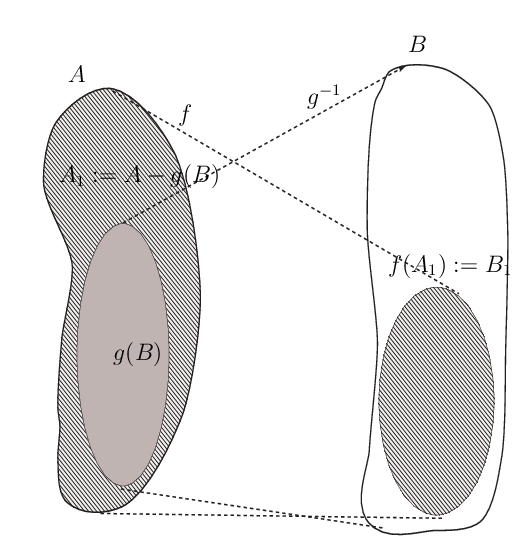
\includegraphics[scale=.5]{imagenes/supfyg.png}
\end{center}

 \caption{Las funciones $f$ y $g^{-1}$}\label{figura3}
\end{figure}

Una primera aproximación sería intentar la construcción
con $\tilde{A}=g(B)^c$. Seguramente así la función
$\tilde{f}$, ver ~\eqref{ftilde}, está bien definida. La
función $\tilde{f}$ será suryectiva, pues $g^{-1}$ es
suryectiva de $g(B)$ en $B$. No obstante, con esa elección de
$\tilde{A}$, la función $\tilde{f}$ no es inyectiva pues cada
elemento de $B_1$ es imágen, por esta $\tilde{f}$, de dos
elementos, uno en $A_1$ y otro en $g(B)$. De modo que esta
elección de $\tilde{A}$ todavía no nos sirve. Lo que vamos
a hacer ahora es agregarle a $\tilde{A}$ el conjunto de todos los
elementos de $g(B)$ tales que $g^{-1}$ los lleva a $B_1$. Este
conjunto es $A_2:=g(B_1)$. Definamos además $B_2:=f(A_2)$. Ahora
$\tilde{f}$ llevará $A_1\cup A_2$ en $B_1\cup B_2$. Nos
preguntamos, ahora, si la elección $\tilde{A}:=A_1\cup A_2$ nos
servirá. Lamentablemente, la respuesta es
no\footnote{Podría ser que si, si la función $f$ hubiera
sido biyectiva desde un principio, cosa que descartamos}. Al haber
agrandado $\tilde{A}$ también se nos agrandó el conjunto
de puntos en $B$ que son imagen de dos puntos, antes era el $B_1$,
ahora apareció el $B_2$. De modo que continuamos el proceso,
es decir, definimos $A_3:=g(B_2)$, $B_3:=f(A_3)$ y así
sucesivamente, ver Figura \vref{figura4} . Nunca llegaremos, en
una cantidad finita de pasos, al conjunto $\tilde{A}$ con la
propiedad deseada, puesto que al cabo de $n$ pasos se nos genera
el conjunto $B_n$ donde las imagenes continuan superponiendosé.
?`Qué haremos entonces?. Lo que se hará es seguir este proceso
indefinidamente, generando una sucesión de conjuntos $A_n$ y
$B_n$, y luego definir:

\begin{equation}\label{defatilde}
\tilde{A}:=\bigcup_{n=1}^{\infty}A_n.
\end{equation}


\index[personas]{Schr\"oder}\index[personas]{Berstein}
\begin{figure}[h]
 \begin{center}
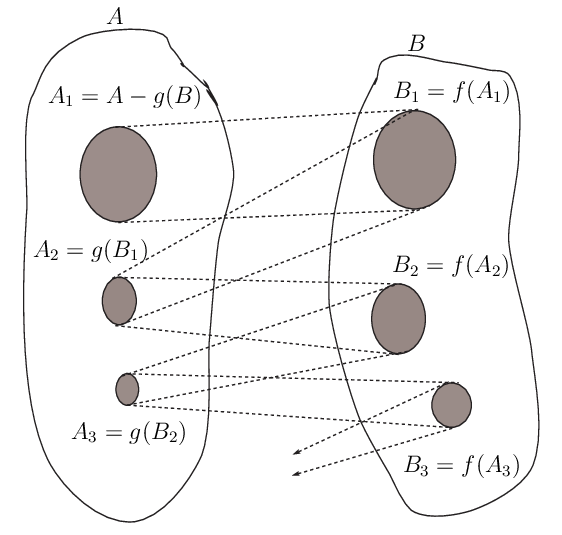
\includegraphics[scale=.5]{imagenes/schber4.png}
\end{center}
 \caption{Demostración del teorema de Schr\"oder-Berstein}\label{figura4}
\end{figure}

Intuitivamente, este conjunto debería  funcionar, es decir no
hay más superposición de $f$ con $g^{-1}$. Esto es pues si
$a\in\tilde{A}$ entonces $a\in A_n$, para algún $n$, y $f(a)\in
B_n$; eventualmente $f(a)$ podría ser igual a algún
$g^{-1}(a')$, pero $a'$ tendría que estar en $A_{n+1}$ y por
consiguiente está en $\tilde{A}$. Y así
$\tilde{f}(a')=f(a')$, y no $\tilde{f}(a')=g^{-1}(a')$, evitando
la superposición de imagenes.

\vspace{10pt}
\begin{demo}\emph{Teorema \ref{scho-ber}} Estamos en condiciones de hacer la demostración propiamente
dicha del teorema. Hasta ahora solo tratamos de explicar la
demostración. Definimos inductivamente conjuntos $A_n$ y $B_n$
de la siguiente manera:

\[\left\{%
\begin{array}{ll}
    A_1=g(B)^c, & B_1=f(A_1) \\
    A_{n+1}=g(B_n), & B_{n+1}=f(A_{n+1}) \\
\end{array}%
\right..\]

Definamos $\tilde{A}$  como en ~\eqref{defatilde} y $\tilde{f}$
como en ~\eqref{ftilde}. Veamos que $\tilde{f}:A\longrightarrow B$
es biyectiva, empezando por la inyectividad.

Sean $a,a'\in A$ dos puntos cualesquiera tales que
$\tilde{f}(a)=\tilde{f}(a')$. Si $a$ y $a'$ están
simultaneamente en $\tilde{A}$, o en $\tilde{A}^c$, tenemos que
$a=a'$ como consecuencia de que $f$ y $g^{-1}$ son inyectivas.
Consideremos entonces el caso $a\in\tilde{A}$ y $a'\notin
\tilde{A}$. Debemos llegar a una contradicción pues estamos
suponiendo indirectamente que $a\neq a'$, por estar en conjuntos
disjuntos, y que $\tilde{f}(a)=\tilde{f}(a')$. Tenemos que, para
algún $n\in\nn$, $a\in A_n$. Además, por la definición de
$\tilde{f}$,  $f(a)=g^{-1}(a')$. Por consiguiente
$g(f(a))=a'$. Como $a\in A_n$, $f(a)\in B_n$ y $a'=g(f(a))\in
A_{n+1}$. Esto contradice que $a'\notin\tilde{A}$.

Veamos ahora la suryectividad. Sea $b\in B$ cualquier punto. Si
$b\in B_n$, para algún $n$, como $B_n=f(A_n)$, ciertamente
existe un elemento $a\in A_n$ tal que $f(a)=b$. Ahora, por la
definición de $\tilde{f}$, $\tilde{f}(a)=f(a)=b$. Supongamos,
pues, que $b$ no está en ningún $B_n$. Como una afirmación
intermedia, probaremos que $g(b)$ no está en ningún $A_n$.
Supongamos, por el contrario, que existe un $n$ tal que $g(b)\in
A_n$. Tiene que ser $n>1$, pues $A_1=g(B)^c$ y $g(b)\in g(B)$.
Así, por su definición  y como $n>1$, el conjunto $A_n$ es
igual a $g(B_{n-1})$. De modo que $g(b)\in g(B_{n-1})$. Esto
implica que existe un $b'\in B_{n-1}$ tal que $g(b)=g(b')$. Pero,
como $g$ es inyectiva $b=b'$ y, por ende, $b\in B_{n-1}$.
Contradiciendo esto que $b$ no estaba en ningún $B_n$. Probamos,
así, que $g(b)$ no está en ningún $A_n$. Por lo tanto
$\tilde{f}(g(b))=g^{-1}(g(b))=b$. Vale decir $b=\tilde{f}(a)$ con
$a=g(b)$. Que era lo que queríamos probar.
\end{demo}

\section{Números Cardinales}
\marginnote{\vspace{-4cm}
\begin{center}
 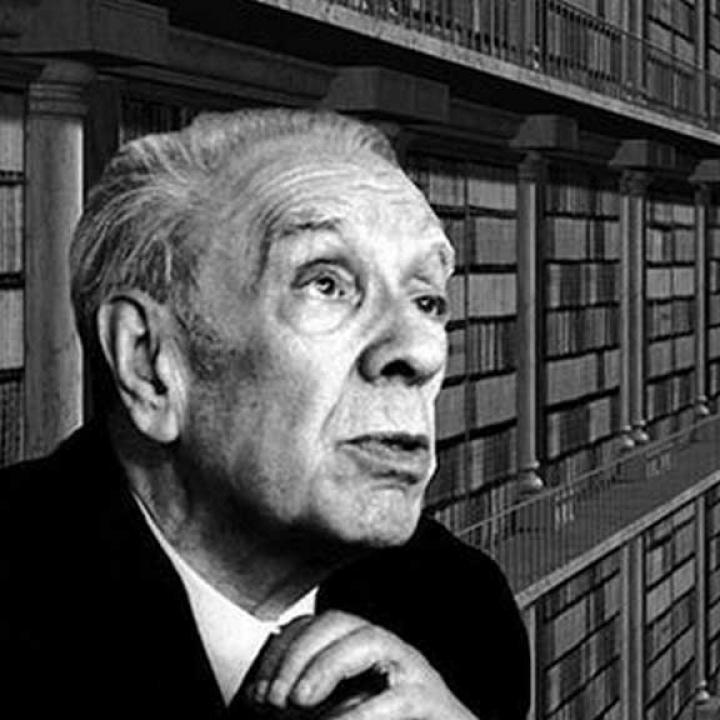
\includegraphics[scale=.13]{imagenes/Borges.jpg}\\
\end{center}
\small
<<Borges y la matemática es un libro de ensayo de 2006 de Guillermo Martínez que relata como varias ideas en la matemática moderna se hallan en la obra literaria del autor argentino Jorge Luis Borges, incluyendo conceptos como la teoría de conjuntos, recursión, la teoría de caos, y sucesión matemática infinita,1​ aunque los enlaces más fuertes que Borges tuvo con la matemática son a través de la teoría de conjuntos infinitos de Georg Cantor. El título del cuento El Aleph se alude al uso de la letra hebrea de Cantor, álef ( $\aleph$ ) por denotar cardinalidad de conjuntos transfinitos>> (Wikipedia)
}

Hasta el momento hemos introducido la noción de cuando dos conjuntos tienen la misma catidad de elementos. Pero no hemos definido el concepto de cantidad de elementos de un conjunto digamos $A$.  A grandes rasgos esto debería ser una característica de todos los conjuntos coordinables con $A$ y se denominará \index{Cardinal}\emph{cardinal} del conjunto $A$ y lo denotaremos por $\#A$. George Cantor defininió este concepto. La definición precisa demanda desarrollar la Teoría de números ordinales, que no es la intención de estas notas. Permítasenos pues invocar el concepto de cardinal a partir de la definición matemáticamente no satisfactoria que dimos, pero creemos que es bastante clara al entendimiento. 

 Se sabe que los números cardinales están ordenados bajo el orden es el definido en la sección anterior.  Concretamente escribiremos   $\#A< \#B$ cuando $A\prec B$. Se puede demostrar que este un buen orden, en el sentido que todo conjunto acotado inferiormente tiene primer elemento. 
 
 Desde George Cantor es costumbre denotar los números cardinales con letras del alfabeto hebreo. Así el primer \emph{cardinal transfinito}\index{Cadinal!transfinito}\footnote{Como es usual adoptaremos la denominación de transfinito en lugar de infinito como usamos hasta aquí} es el que le corresponde a los números naturales y se denota por $\aleph_0$.
 \index[simbolos]{$\aleph_0$} Como el conjunto de cardinales es bien ordenado existe un sucesor de $\aleph_0$ al que denominamos naturalmente $\aleph_1$. Al cardinal que corresponde a los números reales lo denominamos $c$. Sabemos que $\aleph_0<\aleph_1\leq c$ y George Cantor  conjeturó
que $c=\aleph_1$. Esta fue una de las más famosas conjeturas de la matemática y se denominó \href{https://es.wikipedia.org/wiki/Hipótesis_del_continuo}{La Hipótesis del Continuo}. George Cantor fracasó en hallar una demostración de la hipótesis del continuo.   El gran maremático Kurt G\"odel probó en 1938 que esta hipótesis es consistente con el sistema axiomático de la Teoría de conjuntos de  \index[personas]{Zermelo}\index[personas]{Fraenkel} Zermelo y Fraenkel, y por tanto puede ser tomado como un axioma nuevo para la teoría de conjuntos. Sin embargo, en 1963 \index[personas]{Cohen} Paul Cohen probó que la negación de la hipótesis del continuo también es consistente con los axiomas ZF, lo cual prueba que dicha hipótesis es totalmente independiente de los axiomas ZF. Esta situación es similar a la de las geometrías no euclídeas. 
\marginnote{\vspace{-2cm}
\begin{center}
 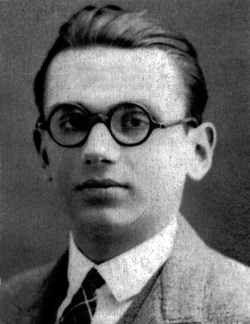
\includegraphics[scale=.3]{imagenes/godel.png}\\
\end{center}
\small
<<Kurt Gödel; Brünn, Imperio austrohúngaro, actual República Checa, 28 de abril de 1906-Princeton, Estados Unidos; 14 de enero de 1978) fue un lógico, matemático y filósofo austríaco.
\newline
Se le considera uno de los lógicos más importantes de todos los tiempos. Su trabajo ha tenido un impacto inmenso en el pensamiento científico y filosófico del siglo XX.  Gödel intentó emplear la lógica y la teoría de conjuntos para comprender los fundamentos de la matemática.
\newline
Se le conoce sobre todo por sus dos teoremas de la incompletitud, publicados en 1931. El más célebre establece que para todo sistema axiomático recursivo auto-consistente lo suficientemente poderoso como para describir la aritmética de los números naturales (la aritmética de Peano), existen proposiciones verdaderas sobre los naturales que no pueden demostrarse a partir de los axiomas. Para demostrar este teorema, desarrolló una técnica denominada ahora numeración de Gödel, que codifica expresiones formales como números naturales.\newline
También demostró que la hipótesis del continuo no puede refutarse desde los axiomas aceptados de la teoría de conjuntos, si dichos axiomas son consistentes. >> (Wikipedia)
}


No contento con introducir los números cardinales transfinitos George Cantor introdujo una aritmética entre ellos. Así por ejemplo si $\aleph_a$ y $\aleph_b$ son dos cardinales, buscamos dos conjuntos disjuntos cualesquiera $A$ y $B$ tales que $\#A=\aleph_a$ y $\#B=\aleph_b$ y definimos
\[
 \begin{split}
  \aleph_a+\aleph_b&=\#A\cup B\\
\aleph_a\times\aleph_b&=\#A\times B\\
\aleph_a^{\aleph_b}&=\#A^B\\
2^{\aleph_a}&=\#2^A
 \end{split}
\]
Algunas relaciones que hemos demostrado
\[
 \begin{array}{ccl}
  \forall \aleph: 2^\aleph &< \aleph & \text{(Por Teorema \ref{teorcantor})}\\  
   \aleph_0\times\aleph_0&=\aleph_0 &\text{(Por Proposición \ref{NxNesnum})}\\
   \aleph_0+\aleph_0&=\aleph_0 &\text{(Por Proposición \ref{unionnumdenum})}\\
   
 \end{array}
\]



\section{Aplicaciones del Teorema de Schr\"oder-Berstein}

El teorema de Schr\"oder-Berstein es una herramienta potente para
probar coordinabilidad de conjuntos puesto que nos permite establecer coordinabilidad mostrando sólo que existen funciones inyectivas entre los conjuntos.

Habíamos visto
que $\rr\nsim\nn$. ?` Qué ocurre con $\rr^2$, $\rr^3$,...?
?`Serán estos conjuntos más ``numerosos'' que $\rr$? Esto es:
?`Serán no coordinables con $\rr$?. Recordando que $\#\rr=c$ nos preguntamos si $c<c^2$. La respuesta a esta
pregunta es negativa, es decir $\rr^n\thicksim\rr$ esto es$c^n=c$. Para ver esto
basta demostrar que $(0,1)^2\thicksim (0,1)$. El caso general es
consecuencia del caso $n=2$, usando inducción, el Ejemplo
\vref{rcoord(0,1)} y el Ejercicio \vref{1.2}.

\begin{teorema} $(0,1)^2\thicksim (0,1)$. En otras palabras $c^2=c$. 
\end{teorema}
\begin{demo} Observar que $(0,1)\precsim (0,1)^2$. Para
demostrarlo considerar la función inyectiva $f(x)=(x,1/2)$.

Veamos que $(0,1)^2\precsim (0,1)$. Debemos construir una
función inyectiva $f:(0,1)^2\longrightarrow (0,1)$. Sea
$(x,y)\in (0,1)^2$. Consideremos las expresiones decimales
$x=0.x_1x_2...$ e $y=0.y_1y_2...$, donde $x_i$ e $y_i$ son enteros
entre 0 y 9, y no son todos 9 a partir de un momento en adelante.
Entonces escribimos:
\[f(x,y):=0.x_1y_1x_2y_2....\]
Es decir $f$ intercala las expresiones decimales de $x$ e $y$.
Esta función es inyectiva, puesto que dos expresiones decimales
iguales tienen todos sus dígitos correspondientes iguales.
Esto concluye la demostración.
\end{demo}

Es bueno notar que la función $f$, definida en la demostración
anterior, no es suryectiva. Un número que no es imagen de
ningún par es $0.909090...$. ?`Por qué será esto?

Por el Teorema \vref{teorcantor} tenemos que
$\nn\prec\mathcal{P}(\nn)$. Desmostramos, además, que $\nn\prec
\rr$. Nos preguntamos, ahora, que relación unirá
$\mathcal{P}(\nn)$ con $\rr$. Con el siguiente teorema probaremos
que aquellos conjuntos son coordinables.

\begin{teorema} $\mathcal{P}(\nn)\thicksim\rr$. En otras palabras $2^{\aleph_0}=c$.
\end{teorema}
\begin{demo} Probaremos que $\mathcal{P}(\nn)\precsim\rr$ y después que
$\mathcal{P}(\nn)\succsim\rr$.

 Como $\mathcal{P}(\nn)\thicksim\mathbf{2}^{\nn}$ ( Ejercicio \vref{6}), y por el
 Ejercicio \vref{1.2} inciso 4, probaremos que $\mathcal{P}(\nn)\precsim\rr$ si podemos
 probar que $\mathbf{2}^{\nn}\precsim \rr$. Para este fin,
 consideremos la siguiente función:
 \[
    \begin{split}
          T:\mathbf{2}^{\nn}&\longrightarrow \rr\\
           f&\longmapsto 0.f(1)f(2)f(3)...\\
    \end{split}
 .\]
Esto es la función $f$ se aplica en un número cuya expansión
decimal tiene solo ceros y unos. Esta función es inyectiva, pues
si
\[0.f(1)f(2)f(3)...=0.g(1)g(2)g(3)...\]
Entonces, por la unicidad de la expansión
decimal\footnote{Recordemos que puede haber expresiones decimales
distintas que representan el mismo número, estas son las
expresiones que tienen todos nueves a partir de un momento en
adelante, como por ejemplo 1=0.999....No obstante este problema no
se nos presenta aquí pues la expresiones decimales que
consideramos tienen solo 0 y 1}, tenemos que $f(1)=g (1)$,
$f(2)=g(2)$,.... Por consiguiente las funciones son iguales. Lo
que prueba la inyectividad. De este modo demostramos que
$\mathbf{2}^{\nn}\precsim \rr$ y esto, por lo que explicamos
anteriormente, implica que $\mathcal{P}(\nn)\precsim \rr$

Ahora debemos ver que $\mathcal{P}(\nn)\succsim\rr$. Utilizando
los  incisos 1. y 4. del Ejercicios \vref{1.2}, vemos que es
suficiente probar que $\rr\precsim \mathcal{P}(\mathbb{Q})$. Para
hacer esto definimos la siguiente aplicación:
\[
   \begin{split}
        T:\rr &\longrightarrow \mathcal{P}(\mathbb{Q})\\
        r &\longmapsto \{q\in\mathbb{Q}:q<r\}
   \end{split}
.\]

Veamos que  la aplicación es inyectiva. Sean $r_1,r_2\in\rr$
números reales distintos, supongamos $r_1<r_2$. Por la densidad
de $\mathbb{Q}$, existe un $q_0\in\mathbb{Q}$ tal que
$q_0\in(r_1,r_2)$. Así $q_0\in\{q\in\mathbb{Q}:q<r_2\}$ y
$q_0\notin\{q\in\mathbb{Q}:q<r_1\}$. De modo que
\[\{q\in\mathbb{Q}:q<r_1\}\neq\{q\in\mathbb{Q}:q<r_2\}.\]
Es decir $T$ es inyectiva.
\end{demo}
Para finalizar demostraremos que
$\nn^{\nn}\thicksim\mathbf{2}^{\nn}$. Mas que el resultado en
sí, vamos a resaltar su demostración, pues contiene una
idea interesante.

\begin{proposicion} $\nn^{\nn}\thicksim\mathbf{2}^{\nn}$. En lenguaje de cardinales  $\aleph_0^{\aleph_0}=2^{\aleph_0}$.
\end{proposicion}

\begin{demo} Dado un conjunto $X$ cualquiera, podemos interpretar una
función $f\in X^{\nn}$ como una sucesión de elementos de $X$,
a la que podemos disponer de la siguiente manera:
\begin{equation}\label{mensajes}
     f=(f(1),f(2),f(3),...).
\end{equation}
Si $X=\nn$ entonces la sucesión será de números naturales y
si $X=\mathbf{2}$ entonces la sucesión será de ceros y unos.

Interpretemos el segundo miembro de ~\eqref{mensajes}  como una
palabra infinita. Si $X=\nn$, esta palabras se compone de
``letras'' que pueden ser cualquier número natural. Si
$X=\mathbf{2}$, esta ``palabra'' se escribe con solo dos
``letras'' el 0 y el 1. La pregunta es: ?`Cómo podemos
``traducir'' una palabra escrita con un alfabeto de infitas
letras, a uno con solo dos?. La solución a esto es ingeniosa.
Sea $f\in\nn^{\nn}$, usaremos el signo 1 para denotar las comas en
la sucesión $f$ y pondrémos tantos ceros como indiquen las
cantidades $f(j)$.


\[
  \begin{split}
         T\quad:\quad\nn^{\nn}\quad\quad &\longrightarrow\quad\quad\mathbf{2}^{\nn}\\
         f=(f(1),f(2),f(3),...)&\longmapsto
          (\underbrace{0,...,0}_{f(1)\,\,\text{ceros}},1,
          \underbrace{0,...,0}_{f(2)\,\,\text{ceros}},1,....)\\
 \end{split}
\]
Veamos que esta función es inyectiva. Sean $f,g\in\nn^{\nn}$,
con  $f\neq g$. Sea
\[j=\min\{i:f(i)\neq g(i)\}.\]
Tenemos que $f(i)=g(i)$ para $i<j$. Escribamos las dos sucesiones

\[   (\underbrace{0,...,0}_{f(1)\,\,\text{ceros}},1,
         ...,1,\underbrace{0,...,0}_{f(j-1)
          \,\,\text{ceros}},1, \underbrace{0,...,0}_{f(j)\,\,\text{ceros}},1,....)
\]
y
\[   (\underbrace{0,...,0}_{g(1)\,\,\text{ceros}},1,
         ...,1,\underbrace{0,...,0}_{g(j-1)
          \,\,\text{ceros}},1, \underbrace{0,...,0}_{g(j)\,\,\text{ceros}},1,....)
\]
Notar que los primeros $j-1$ grupos de ceros son iguales, pues
$f(i)=g(i)$ para $i<j$, por consiguiente los primeros $j-1$ unos
estan en la misma posición en las dos sucesiones. Pero $f(j)\neq
g(j)$ y, por consiguiente, el grupo $j$-ésimo de ceros debe
diferir en las dos sucesiones. Esto fuerza que si, por ejemplo,
$f(j)<g(j)$, entonces la sucesión $f$ tendrá un uno donde la
$g$ tiene un cero.

Así $T(f)\neq T(g)$ y la función es inyectiva. Esto prueba
que $\nn^{\nn}\precsim \mathbf{2}^{\nn}$. La otra desigualdad es
más fácil de obtener pues
\[
  \begin{split}
      \mathbf{2}&\precsim \nn\quad\,\,\, \text{pues unos es finito y el
      otro no}\\
      \mathbf{2}^{\nn}&\precsim\nn^{\nn}\quad \text{por el
      Ejercicio \ref{potdelapot} }
  \end{split}
\]
\end{demo}

Existe una demostración más sucinta de que
$\nn^{\nn}\precsim\mathbf{2}^{\nn}$. No la preferimos debido a que
no muestra una biyección, es una demostración indirecta. Ahora
la exponemos.
\[
  \begin{split}
       \nn &\precsim \mathbf{2}^{\nn}\quad\quad\,\text{Teorema de
       Cantor}\\
       \nn^{\nn} &\precsim (\mathbf{2}^{\nn})^{\nn}\quad\text{Ejercicio
       \ref{potdelapot}}\\
        \nn^{\nn} &\precsim \mathbf{2}^{\nn\times\nn}\quad\,\text{Ejercicio
       \ref{potdelapot}}\\
        \nn^{\nn} &\precsim \mathbf{2}^{\nn}\quad\quad\,\text{Proposición  \ref{NxNesnum}}\\
        \nn^{\nn} &\precsim \mathbf{2}^{\nn}\quad\quad\,\text{Ejercicio
       \ref{1.2} inciso 3}.
  \end{split}
\]


\section{Ejercicios}


\begin{ejercicio}\label{propuniarb} Sea $f:A\longrightarrow B$ una función cualquiera.
Supongamos que $\{A_i\}_{i\in I}$ y $\{B_i\}_{i\in I}$ son
familias subindicadas de conjuntos, donde los $A_i$ y $B_i$ son
subconjuntos de $A$ y $B$ respectivamente. Demostrar las
siguientes propiedades:
\end{ejercicio}
\begin{itemize}
\item[1.] $\biggl(\bigcup_{i\in I}A_i\biggr)^c=\bigcap_{i\in
I}A_i^c$.
\item[2.]$\biggl(\bigcap_{i\in I}A_i\biggr)^c=\bigcup_{i\in
I}A_i^c$.
\item[3.] $f\biggl(\bigcup_{i\in I}A_i\biggr)=\bigcup_{i\in
I}f(A_i)$.
\item[4.]?`Qué ocurre con $f\biggl(\bigcap_{i\in I}A_i\biggr)$?
\item[5.] $f^{-1}\biggl(\bigcup_{i\in I}B_i\biggr)=\bigcup_{i\in
I}f^{-1}(B_i)$.
\item[6.]$f^{-1}\biggl(\bigcap_{i\in I}B_i\biggr)=\bigcap_{i\in
I}f^{-1}(B_i)$.
\end{itemize}

\begin{ejercicio}\label{3} Demostrar las propiedades de la
Proposición \vref{propfunc}
\end{ejercicio}
\begin{ejercicio}\label{1} Probar que $\thicksim$ es una
relación de equivalencia.
\end{ejercicio}
\begin{ejercicio}\label{1.2} Supongamos que $A\thicksim B$ y
$C\thicksim D$.
\begin{itemize}
\item[1.] Demostrar que $\mathcal{P}(A)\thicksim \mathcal{P}(B)$.
\item[2.] Demostrar que $A\times C\thicksim B\times D$.
\item[3.] Demostrar que $A^C\thicksim B^D$.
\item[4.] Si $A\precsim C$ entonces $B\precsim D$.
\end{itemize}
\end{ejercicio}
\begin{ejercicio}\label{potdelapot} Sean $A$, $B$ y $C$ conjuntos
no vacios. Demostrar que
\begin{itemize}
\item[1.] $\bigl(A^{B}\bigr)^C\thicksim A^{B\times C}$.
\item[2.] Si $A\precsim B$ entonces $A^C\precsim B^C$.
\end{itemize}
\end{ejercicio}

\begin{ejercicio}\label{1.5} Demostrar que un subconjunto de un conjunto
finito es finito.
\end{ejercicio}
\begin{ejercicio}\label{2} Demostrar que la función
$f:\nn\times\nn\longrightarrow\nn$ definida por:
\[f(j,k):=\frac{(j+k-1)(j+k)}{2}-j+1,\]
es una biyección.
\end{ejercicio}
\begin{ejercicio}\label{5} Demostrar, exhibiendo una biyección, que $(0,1)\thicksim [0,1]$
\end{ejercicio}
\begin{ejercicio}\label{6} Demostrar que el conjunto
$\mathcal{P}(\nn)$ es coordinable con el conjunto
$\mathbf{2}^{\nn}$, donde $\mathbf{n}=\{0,1,...,n-1\}$. Recordar
que, si $A$ y $B$ son conjuntos, $B^A:=\{f:f:A\longrightarrow
B\}$. De este modo $\mathbf{2}^{\nn}$ es el conjunto de funciones
$f:\nn\longrightarrow \{0,1\}$.
\end{ejercicio}

\begin{ejercicio}\label{8} Demostrar que, para cualquier conjunto
$A$, $\mathcal{P}(A)\thicksim\mathbf{2}^A$.
\end{ejercicio}
\begin{ejercicio}\label{infcoordconsub} Demostrar que son
equivalentes:
\begin{itemize}
     \item[1.] $A$ es infinito.
     \item[2.] $A$ es coordinable con un subconjunto propio, es
     decir: Existe $B\subset A$, con $B\neq A$, tal que
     $A\thicksim B$.
\end{itemize}
\end{ejercicio}
\begin{ejercicio} Demostrar que el conjunto formado por todos los
sub-\newline conjuntos de $\nn$ que son finitos, es numerable.
?`Qué ocurrira con el conjunto de todos los subconjuntos
infinitos?
\end{ejercicio}
\begin{ejercicio} Sea $\{A_i\}_{i\in I}$ una familia de intervalos
de $\rr$. Suponer que los conjuntos en la familia son mutuamente
disjuntos, es decir: $A_i\cap A_j=\emptyset$ si $i\neq j$.
Demostrar que el conjunto $\{A_i:i\in I\}$ es a lo sumo numerable.
\end{ejercicio}
\begin{ejercicio} Recordemos que una función
$f:\rr\longrightarrow\rr$ se dice nodecre-\newline ciente, si para
todos $x,y\in\rr$, tales que $x<y$, se tiene que $f(x)\leq f(y)$.
Dada una función nodecreciente, demostrar que el conjunto de
todos los puntos de discontinuidad es a lo sumo numerable.
\textit{Ayuda}: Demostrar en primera instancia que los
límites laterales:
\[
    \lim\limits_{x\rightarrow a^+}f(x)\quad\text{y}\quad \lim\limits_{x\rightarrow
    a^-}f(x)
\]
existen para todo $a\in\rr$. Luego aplicar el ejercicio anterior.
\end{ejercicio}
\begin{ejercicio} Demostrar que $\rr^{\nn}\thicksim\rr$.
\end{ejercicio}
\begin{ejercicio} Como aprendimos $\nn\thicksim\mathbb{Q}$, esto
significa que existe una aplicación biyectiva
$f:\nn\longrightarrow\mathbb{Q}$, que nos permite enumerar
$\mathbb{Q}$ como una suceción $r_j:=f(j)$. Definimos la
aplicación:
\[\begin{split}
              T:C(\rr)&\longrightarrow \rr^{\nn}\\
              f        &\longmapsto T_f\\
\end{split}\]
donde
\[
  T_f(j):=f(r_j).
\]
\begin{itemize}
   \item [1.] Demostrar que $T$ es inyectiva. Por consiguiente
   $C(\rr)\precsim\rr^{\nn}$.
   \item[2.] Usando el inciso anterior, demostrar que
    $C(\rr)\thicksim\rr$, donde $C(\rr)$ es el conjunto
    de las funciones continuas de $\rr$ en si mismo.
\end{itemize}
\end{ejercicio}
